\subsubsection{聚类簇包特征}
我们首先对所有词向量进行聚类操作,然后对每个词,按其所在簇的中心编号对这个词进行标记。
得到的词的特征是簇编号的集合,这样语义上相似的词会有同样的特征。\\
我们最后使用的特征和词包的思想类似,用簇包来表征文本的特征。
也就是说将文本中的每个词替换成它所在簇的编号,然后对这个新构成的“文本”构造“词包”特征,就是我们的“簇包“特征。
利用上述方式构造的簇包特征来训练分类器,得到如下图\ref{fig:3cword2veccluster}所示的结果:
\begin{figure}[h]
\centering
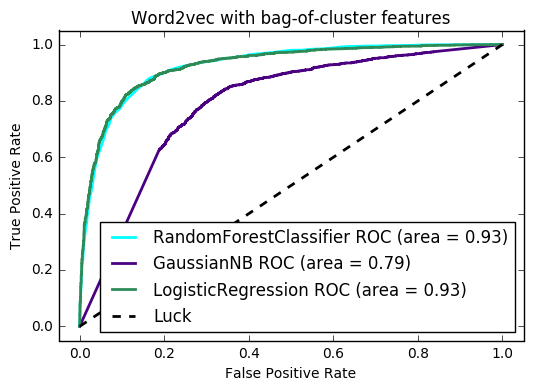
\includegraphics[width=0.9\linewidth]{3c_word2vec_cluster}
\caption[word2vec_cluster]{三种模型用Word2vec的簇包特征的ROC曲线}
\label{fig:3cword2veccluster}
\end{figure}

可以看到结果比使用平均词向量特征的模型要好一点点,但其实在误差范围内并没有改进。\\
理论上来讲,聚类簇包特征已经兼顾了文本的统计信息和语义信息,构造出的特征集信息量更大。
在其上进行分类,应该会得到更优的结果。
然而在这个实验里却没有明显的改进。\\
一种可能的原因是统计信息或者语义信息对于分类的作用已经被我们穷尽,所以局限在这两个领域内的特征对于分类都没有明显的提升作用。
另一种原因是我们仍没有完全发掘文本的统计或者语义特征,例如对于平均词向量特征而言,我们可以使用之前提到的TF-IDF进行加权平均。而词向量模型也可以用更多更全的语料库进行训练。